\chapter{
    Time Frame
    \\
    \large{Fine Tuning The Model}
}
\label{sec:TimeFrame}

Section \ref{sec:PotentialSurfaceLinearRegressionAndTimeSeriesProblems} introduced the notion of a time frame, or a window of time over which data is selected to use for linear regression. This is important because it allows the model to track changes over time. The natural question then becomes how long should the time frame be, and is what this section is concerned with.

Figure \ref{fig:Pred1RMMultipleTimeFrames} shows how the predicted 1RM changes over time with varying time frames. It should be clear that the time frame chosen has a significant impact on what predictions the model makes, and as such will need to be chosen so that it increases the accuracy of the model. This will require first defining the models accuracy, and then later using that definition to choose a time frame such that the models accuracy is maximized.

\begin{figure}[h]
    \centering
    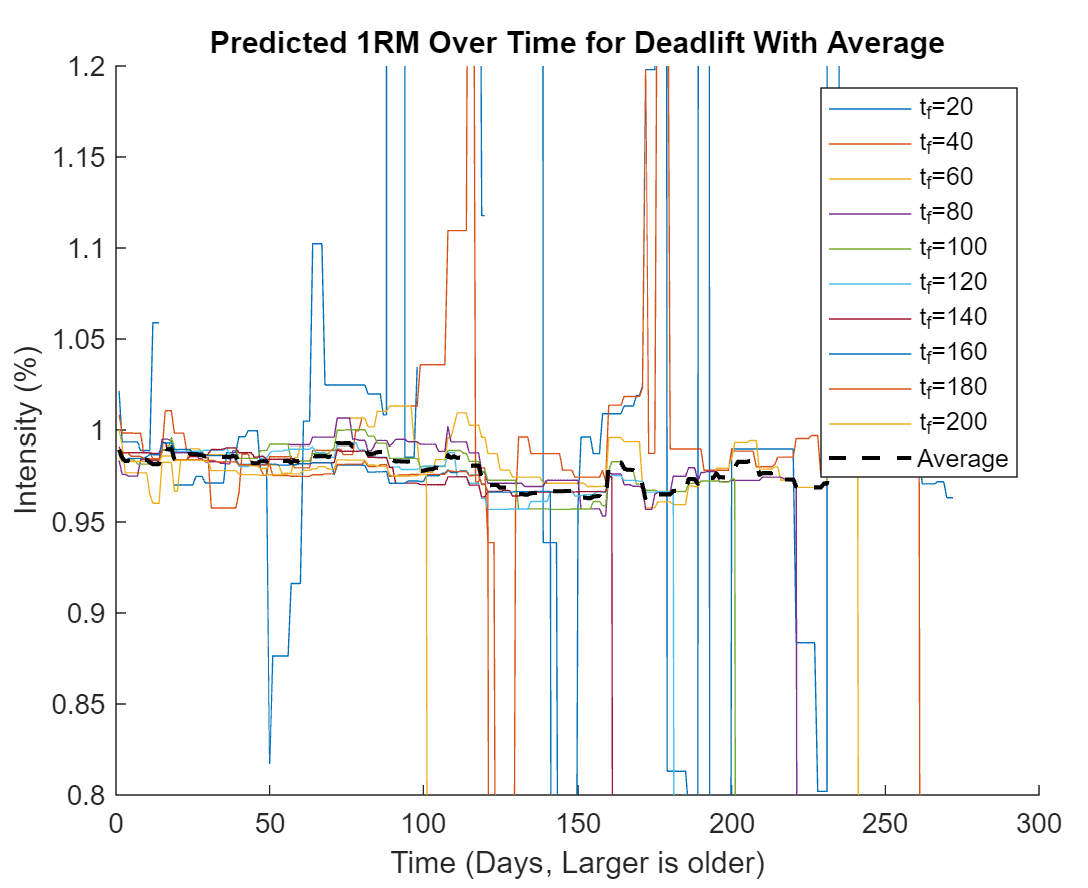
\includegraphics{DeadliftConstants/pred1RMMultipleTimeFrames.png}
    \caption{The models predicted 1RM over varying time frames. The large spikes and dips are from the model not having enough data to fit the fatigue aware potential surface to. The $20$ and $40$ time frames were excluded from calculating the average due to there erratic and inaccurate behavior.}
    \label{fig:Pred1RMMultipleTimeFrames}
\end{figure}

\section{Establishing Lose Bounds}
\label{sec:TimeFrameEstablishingLooseBounds}

The first thing to take note of from figure \ref{fig:Pred1RMMultipleTimeFrames} is the $20$ and $40$ day time frames, as they have large spikes and drops. This is the result of the model not having enough data. Given that the lifter performed deadlifts at most $2$ times a week, this creates a maximum of $11$ data points for linear regression to use over a $40$ day time frame. This is not enough data for the model to accurately predict anything. The time frame chosen needs to be large enough for the model to have enough data to reliably create predictions. With this in mind, the 1RM prediction has presented itself as a proxy to determine if the model was given enough data. If the 1RM prediction is within 'reasonable' bounds then it can be presumed that the model was given enough data to make accurate predictions. This is not an exact measurement to determine if the model has been given enough data, but is a proxy that can help avoid situations where the model was clearly not given enough data.

Looking at the larger time frames the behavior is much more stable, but at the cost of requiring more data to create any predictions. If a time frame is to large it will fail to adapt to recent changes in a lifters abilities, as it includes old data that may no longer be relevant to a lifters current capabilities. It should be clear that when considering a time frame, a balance needs to be struck so that the model has enough data to be reliable but not to much data so that it fails to capture recent changes in a lifters abilities.

\section{Accuracy: Defining State and What is Being Measured}
\label{sec:TimeFrameWhatIsBeingMeasured}

The 1RM prediction has already been introduced as a measure of accuracy in sections \ref{sec:PotentialSurfaceSolvingForTheUnknown}, \ref{sec:PotetentialSurfaceImprovingAccuracy}, and just now in section \ref{sec:TimeFrameEstablishingLooseBounds}. However, this is only a single data point from the output of the model. Accuracy can, and probably should, be considered in a much larger context. From equations \ref{eq:PotentialSurfaceSetsEquationWithFatigue}-\ref{eq:PotentialSurfaceFatigueEquation}, it can be presumed that the model can predict sets, reps, effort, intensity, and fatigue.

\begin{wrapfigure}{l}{0.55\textwidth}\centering
    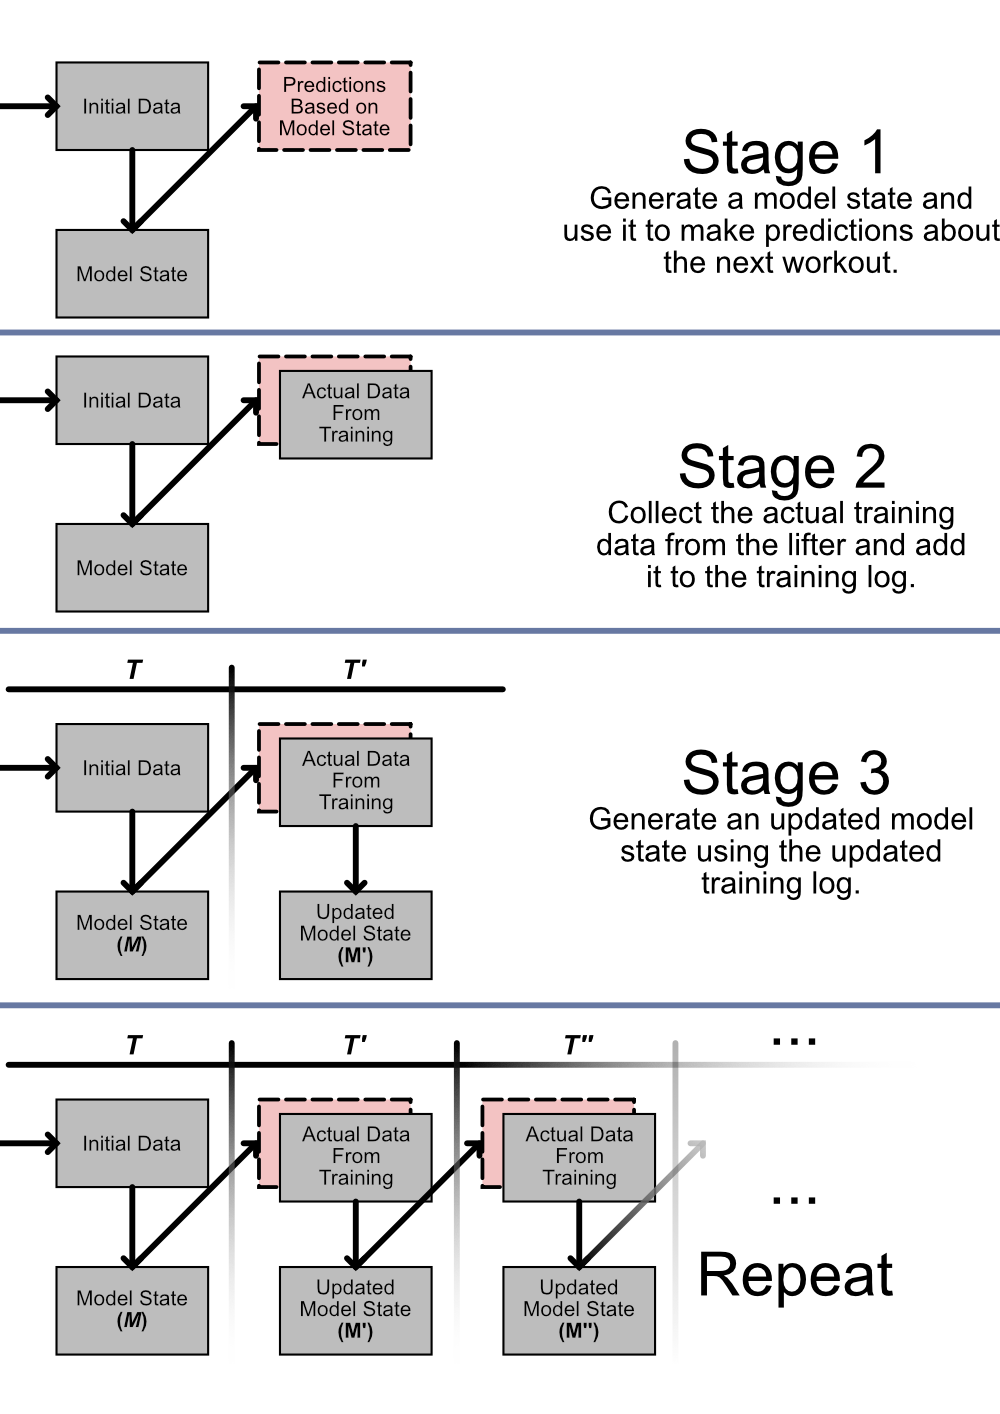
\includegraphics[width=95mm]{Diagrams/PredictionsDiagram.png}
    \caption{A diagram showing how the model makes predictions through time.}
    \label{fig:ModelPredictionsDiagram}
\end{wrapfigure}

Before any discussion about measuring accuracy, it is worth describing how the model predicts values. If the model is predicting a value for the current day, then it will use historical data that is within the selected time frame, $t_i\in\{ t_t=t_0, t_t+1=t_0+1, \dots, t_0+t_f \}$, to create a prediction. Given this specific set of historical data, the model will have a certain state, called the \textit{model state}, which is defined by the set of all constants produced from linear regression, as shown in equation \ref{eq:ModelState}. This definition makes the model state specific to the subset of historical data used, hence the $T$ subscripts, and means that the state of the model will change with any changes to the time frame. This is consistent with the observations made from figure \ref{fig:Pred1RMMultipleTimeFrames}.

\begin{equation}
    \label{eq:ModelState}
    M\in \{ a_{T}, b_{T}, c_{T}, \epsilon_{T}, \epsilon_{2,T} \}
\end{equation}

Once the actual data for a given day is added to the data set, any discrepancies between the predicted and actual data can be used to measure accuracy. When the lifter goes to train the next time, the process can repeat itself all over again, but this time the model will use time frame $T'$ and will be in in state $M'$ because of the data that was added from the previous workout. It is through this mechanism that the model is able to change state as it moves through time, and gives it the ability to adapt to represent the lifters current abilities. Figure \ref{fig:ModelPredictionsDiagram} demonstrates this process in a graphical manner.

The above process of the model updating state as it moves through time is necessary for the model to adapt, but creates challenges when attempting to gather historical data, which can be used to do things like measure accuracy over time. Every time a prediction needs to be made for time $t_t$, the model must use the appropriate time frame to get the state of the model before the data at time $t_t$ was added. Calculating the models state is a non-trivial process, and having to repeat it for every time value results in large computational overhead. Any efficiency that can be gained from calculating the models state will have significant impacts on the speed of generating historical model data.

Now that it is known how the model makes predictions, and hence how to measure accuracy, tools like the mean square error (MSE) and root mean square error (RMSE) can be used to measure accuracy from a larger context. The graphs in table \ref{tab:PredictionsVsActualConstantTimeFrame} show the actual vs predicted values for various variables using deadlift data. The reason there are not predictions for all values is because some values were to close to the end of the data set for the given time frame to make predictions, which brings up an important point: the amount of data the model needs before it can start creating predictions is dependent on the time frame chosen. This limitation will be partially removed in section \ref{sec:TimeFrameDynamicTimeFrameAnalysis}, but cannot be wholly removed because the model will always need a certain amount of data to create reliable predictions, as discussed in section \ref{sec:TimeFrameEstablishingLooseBounds}.

\begin{table}
    \centering
    \begin{tabular}{c|c}
        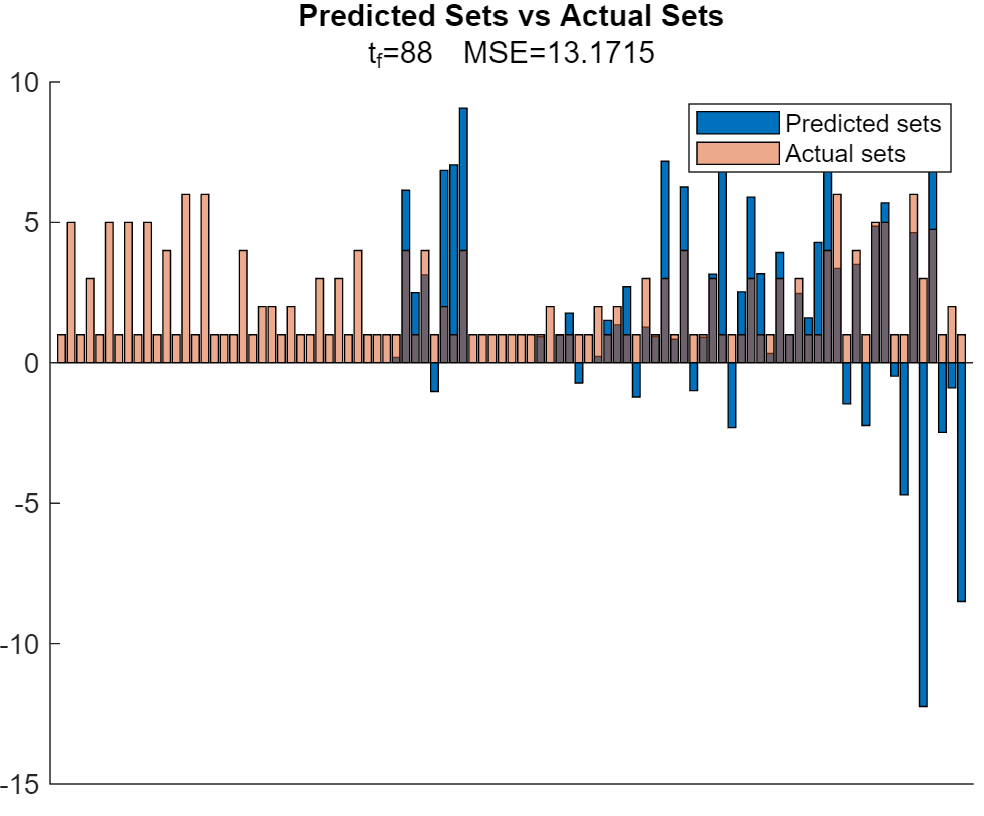
\includegraphics[width=80mm]{ActualVsPredValues/ActualVsPredSets.png} &
        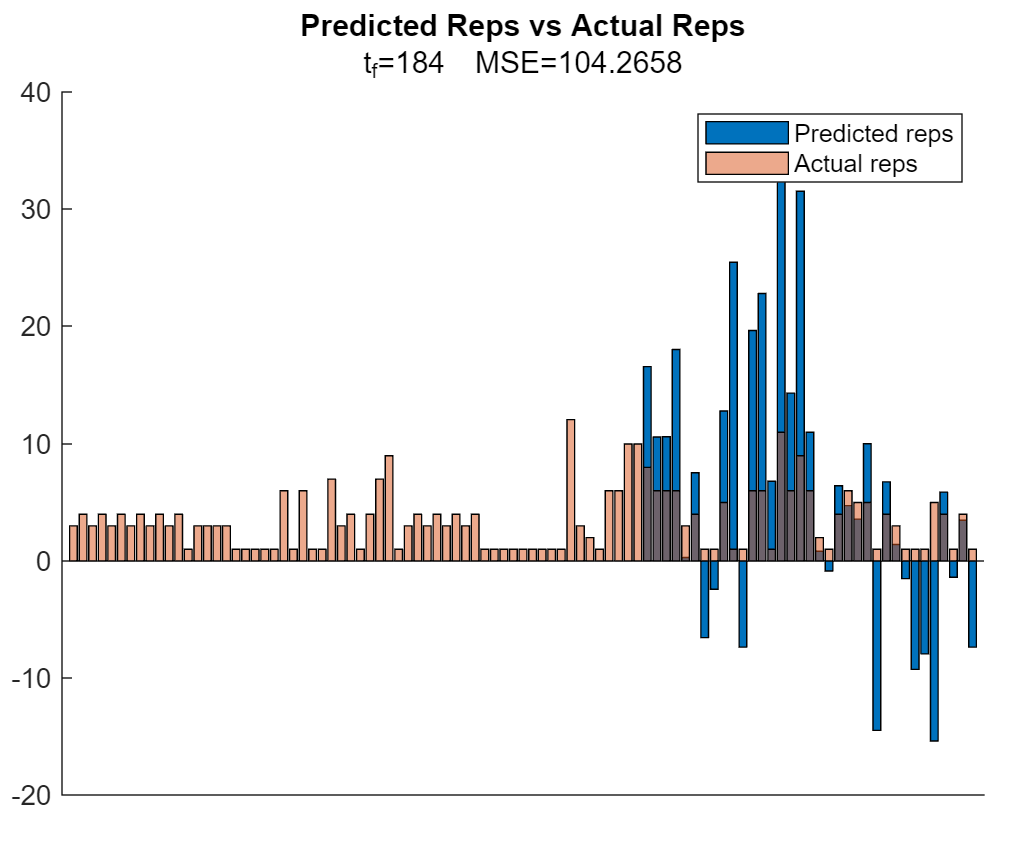
\includegraphics[width=80mm]{ActualVsPredValues/ActualVsPredReps.png}  \\
        
        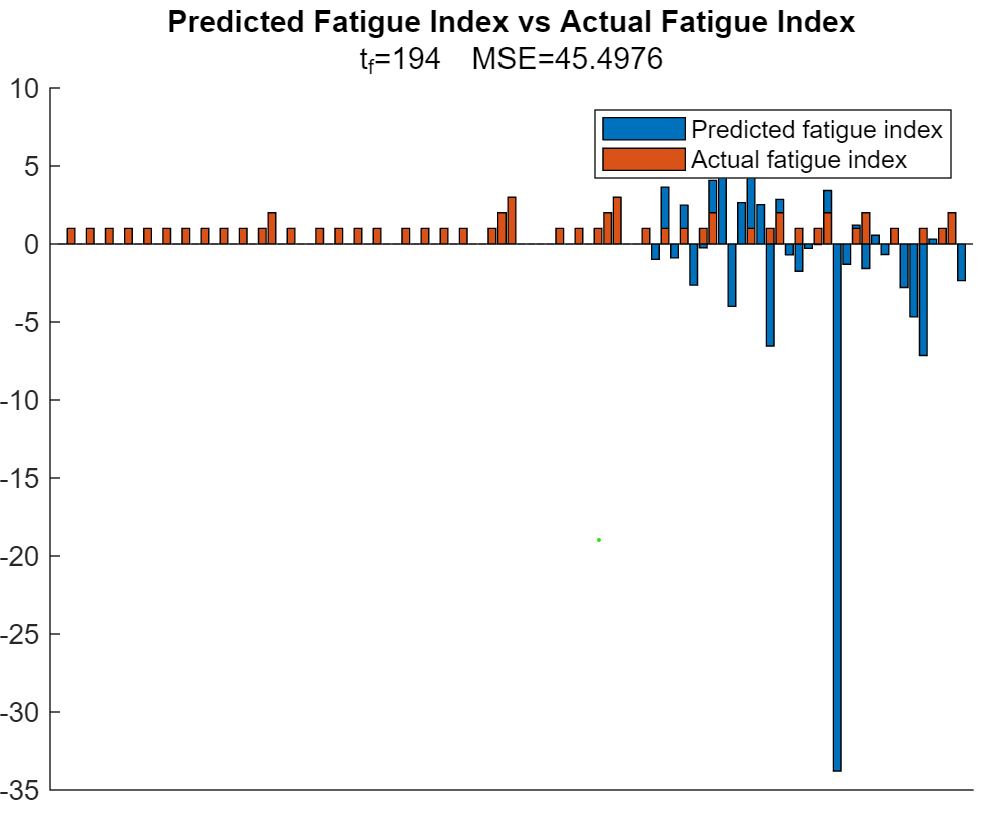
\includegraphics[width=80mm]{ActualVsPredValues/ActualVsPredFatigueIndex.png} &
        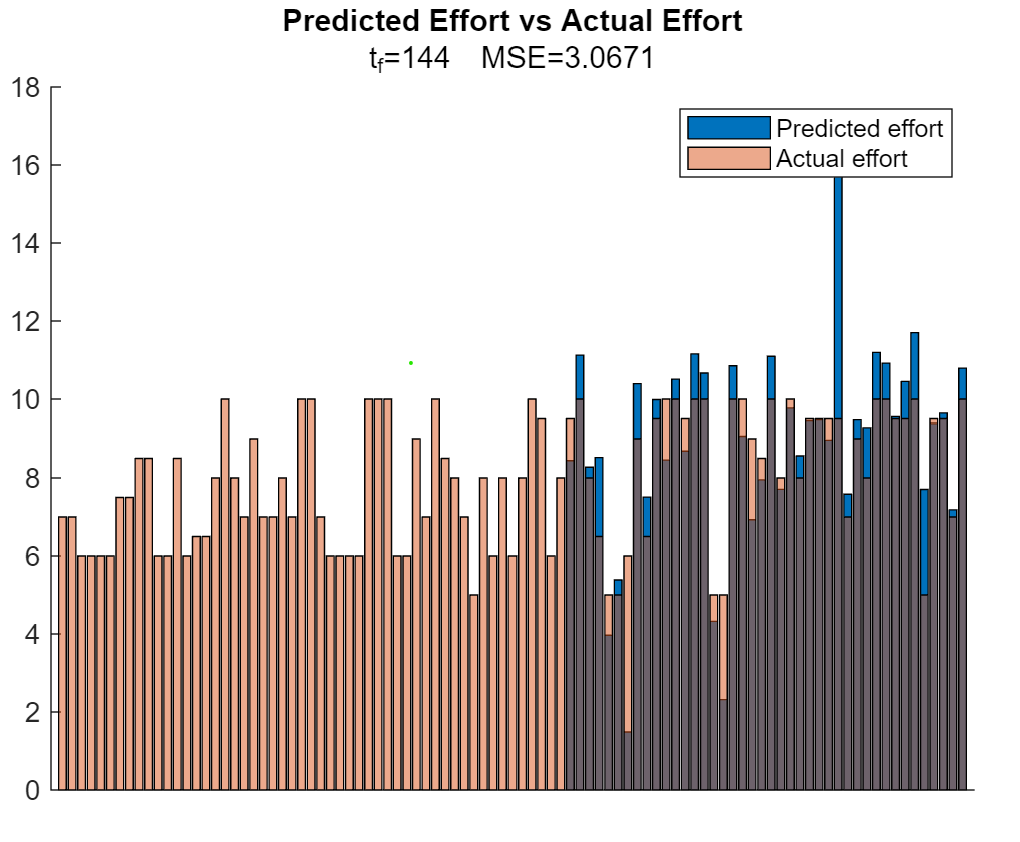
\includegraphics[width=80mm]{ActualVsPredValues/ActualVsPredEffort.png} \\
        
        \multicolumn{2}{c}{
            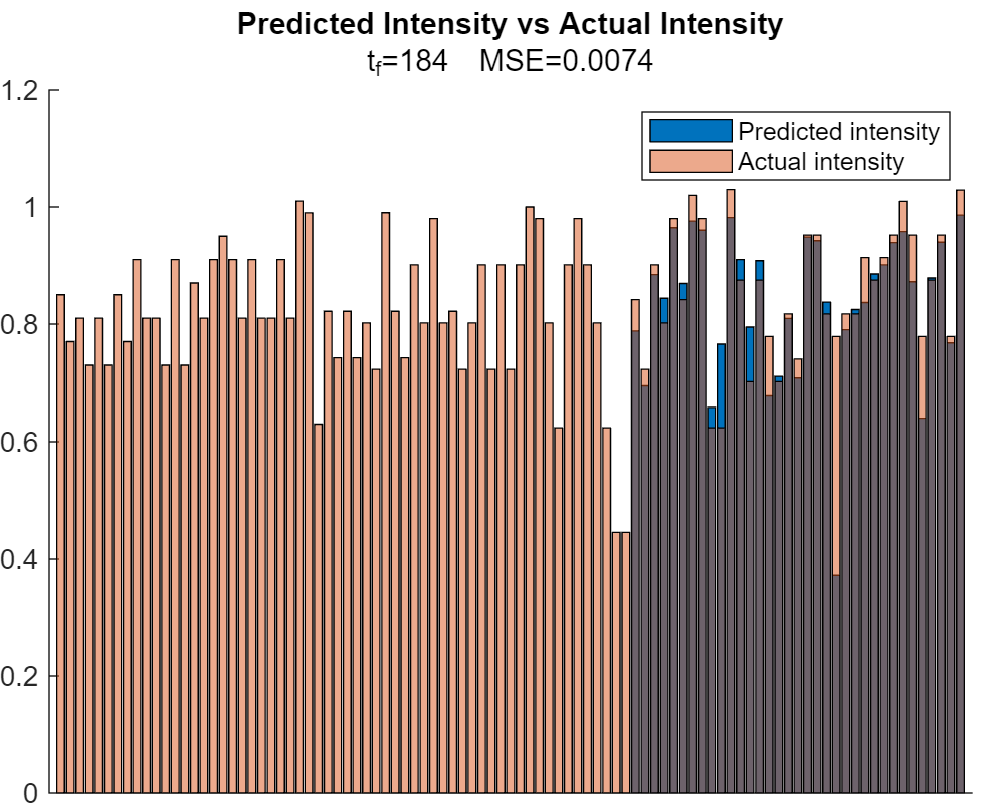
\includegraphics[width=100mm]{ActualVsPredValues/ActualVsPredIntensity.png}
        }
    \end{tabular}
    \caption{Predicted values compared to actual values for various variables using deadlift data. Sets, reps, and the fatigue index are not accurate, but effort is more accurate, and intensity is very accurate. The MSE was calculated only using data points that had a predicted value.}
    \label{tab:PredictionsVsActualConstantTimeFrame}
\end{table}

Some of the graphs from table \ref{tab:PredictionsVsActualConstantTimeFrame} may seem surprising, especially the ones relating to sets, reps, and the fatigue index. The results displayed in these graphs are highly inaccurate. The reason for this is rather simple, in section \ref{sec:PotentialSurfaceDefiningTheRelationships} the error terms that were minimized were in relation to intensity, which defined intensity as the dependent variable. Even before that however, the intuitive relationships discussed in section \ref{sec:PotentialSurfaceIntuitiveRelationshipsBetweenVariables} were all focused on how volume, effort, sets, and reps all affected intensity, which implicitly defined all of those values as independent variables and intensity the dependent variable. So, the reason for the inaccuracy in the set, rep, and fatigue index graphs are because a dependent variable was being predicted from an independent variable, which in the context of modeling does not make sense. This also explains the accuracy of the intensity graph, with the predicted intensity, on average, being within $0.74\%$ of the actual intensity. Moving forward, this means that equations \ref{eq:PotentialSurfaceSetsEquationWithFatigue}, \ref{eq:PotentialSurfaceRepsEquationWithFatigue}, \ref{eq:PotentialSurfaceEffortEquationWithFatigue}, and \ref{eq:PotentialSurfaceFatigueEquation} should all be used sparingly, and when used there results should be questioned. Of note is that equation \ref{eq:1RMPredictionWithFatigue} remains unaffected by this, and means that the 1RM predictions produced by the model should have some accuracy to them.

\section{Choosing A Time Frame: Static Time Frame Analysis}
\label{sec:TimeFrameStaticTimeFrameAnalysis}

A time frame of constant length $t_f$ can be used across all time values to generate predictions, creating a 'static time frame'. With accuracy defined and having shown how the model predicts values, the MSE of intensity across all time values can be used as a way to select a value for $t_f$ that maximizes the accuracy of the model. Figure \ref{fig:StaticTimeFrameDiagram} demonstrates the process of selecting a static time frame.

\begin{figure}[h]
    \centering
    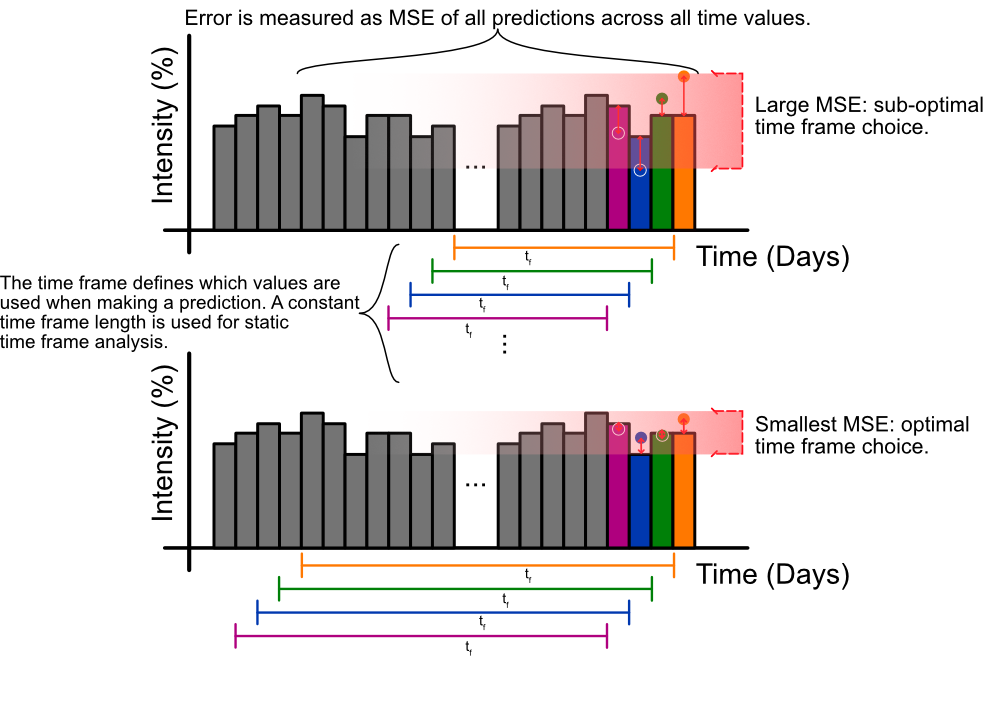
\includegraphics[width=150mm]{Diagrams/StaticTimeFrameDiagram.png}
    \caption{A diagram showing how a static time frame is calculated from the data set. Note how the predictions for all time values need to be recalculated.}
    \label{fig:StaticTimeFrameDiagram}
\end{figure}

The models accuracy will be maximized when the MSE is minimized. In order to find the global minimum MSE, all valid values of $t_f$ must be tested and there respective MSE's calculated. Equation \ref{eq:ValidTimeFrameSet} shows the set that determines all valid values for the time frame given a target time, $t_t$.

\begin{equation}
    \label{eq:ValidTimeFrameSet}
    t_f \in \{ 0, 1, \dots , \max_{t_1\dots t_n}( t )-t_t \}
\end{equation}

The algorithm shown in listing \ref{lst:StaticTimeFrameFormula} can be used to find the $t_f$ value where the MSE is minimized. Given that \texttt{modelState} runs in linear time with it's arguments, which happens because it has to sum up values across it's given time frame, this algorithm has a time complexity of $O(n^3)$. As the lifter keeps lifting and the data set grows $\max_{t_1\dots t_n}(t)$ will continually increase, eventually making an exhaustive search of all $t_f$ values infeasible. An analytical approach to finding the global minimum of the MSE would be nice, but this is not possible as the MSE error function is not a continuous function rendering any method derived from calculus useless. If historical data is needed, the time complexity gets even worse, with listing \ref{lst:HistoricalStaticTimeFrameFormula} showing the that the time complexity of getting historical data is $O(n^4)$.

% \begin{equation}
%     \sum_{t_f\in\{0,1,...,\max_{t_1...t_n}(t)\}}\left(
%         \min\left(
%             \frac{
%                 \sum_{t_{t,i}\in \{ t \; | \; t+t_{f,i}\le \max_{t_1\dots t_n}(t) \; \wedge \; t\le t_t\}}
%                 \left(
%                     intensityPred(modelState(t_{t,i+1},t_{f,i}),s_i,r_i,E_i,F_i)
%                 \right)^2
%             }{
%                 |t_{t,i}\in \{ t \; | \; t+t_{f,i}\le \max_{t_1\dots t_n}(t) \; \wedge \; t\le t_t\}|
%             }
%         \right)
%     \right)
% \end{equation}

\begin{minipage}{\linewidth}
\begin{lstlisting}[caption={The algorithm that describes how to exhaustively find a static time frame's length such that it minimizes the models error.},label={lst:StaticTimeFrameFormula},mathescape=true]
# $s$, $r$, $E$, $F$, and $t$ are all lists of there respective variables
fun staticTimeFrame$(s,r,E,F,t,t_t) \to (t_f, \varepsilon)$
    $t_{f,min}=-1$
    $\varepsilon_{min}=0$
    for each $t_{f,i}\in \{ 1, \dots, \max_{t_1\dots t_n}(t)-t_t \}$
        $\varepsilon=0$
        $\varepsilon_{cntr}=0$
        for each $t_{t,i}\in \{ t \; | \; t+t_{f,i}\le \max_{t_1\dots t_n}(t) \; \wedge \; t\ge t_t\}$
            # The $i+1$ subscript ensures the current data point, the value being
            # predicted, is not part of the model state
            $M=$modelState$(t_{t,i+1},t_{f,i})$
            $I_{pred}=$intesityPrediction$(M,s_i,r_i,E_i,F_i)$
            $\varepsilon=\varepsilon+(I_{pred}-I_{i+1})^2$
            $\varepsilon_{cntr}+=1$
        $\varepsilon/=\varepsilon_{cntr}$
        if $\varepsilon<\varepsilon_{min}$
            $\varepsilon_{min}=\varepsilon$
            $t_{f,min}=t_{f,i}$
    return $( t_{f,min}, \varepsilon )$
\end{lstlisting}
\end{minipage}

\begin{minipage}{\linewidth}
\begin{lstlisting}[caption={The algorithm that describes how to find historical static time frames.},label={lst:HistoricalStaticTimeFrameFormula},mathescape=true]
# $s$, $r$, $E$, $F$, and $t$ are all lists of there respective variables
fun historicalStaticTimeFrames$(s,r,E,F,t) \to \left( [t_{f,1},\dots,t_{f,n}], [\varepsilon_1,\dots,\varepsilon_n] \right)$
    $t_{f,min}=[0, 0, \dots]$ where $|t_{f,min}|=n$
    $\varepsilon_{min}=[0, 0, \dots]$ where $|\varepsilon_{min}|=|t|$
    for each $t_{t,i}\in \{ t \} $
        $(t_{f,min}[i], \varepsilon_{min}[i])=$staticTimeFrame$(s,r,e,F,t)$
    return $(t_{f,min},\varepsilon_{min})$
\end{lstlisting}
\end{minipage}

If the summations used in \texttt{modelState} are saved then a dynamic programming approach can be used to reduce the time complexity of \texttt{modelState} to constant time, reducing the time complexity of listing \ref{lst:StaticTimeFrameFormula} to $O(n^2)$ and listing \ref{lst:HistoricalStaticTimeFrameFormula} to $O(n^3)$. Despite the drastic improvement, these time complexities are still not usable as the data set gets larger.

Without a clear way to further optimize the static time frame algorithm presented in listing \ref{lst:StaticTimeFrameFormula}, the problem needs to be constrained. One way to do this is to only find a local minimum of the MSE. Conceptually, the approach to determine a local minimum of the MSE is not much different from whats outlined in listing \ref{lst:StaticTimeFrameFormula}. Instead of exhaustively searching the entire set of $t_f$ values, the algorithm stops when it finds a minimum. This will result in time savings as long as the MSE is not continually decreasing across the entire range of $t_f$ values.

Another approach to constrain the problem is to simply bound the time frame to always be less than a certain length and only search for a minimum MSE value within a specific range of $t_f$ values. This approach was used to create the graphs in table \ref{tab:PredictionsVsActualConstantTimeFrame}. The MSE values for all $t_f\in \{ 60, 61, ... , 200 \}$ were used, and from this set, the $t_f$ value corresponding with the smallest MSE relative to the variable being predicted was then selected to generate each graph, explaining the different time frame values shown in the table. Figure \ref{fig:MSEStaticTimeFrame} shows the MSE values for every $t_f$ value when intensity was the variable being predicted. It demonstrates the non-continuous nature of the MSE, and demonstrates the obvious fact that the first minimum is not guaranteed to be the global minimum.

\begin{figure}[h]
    \centering
    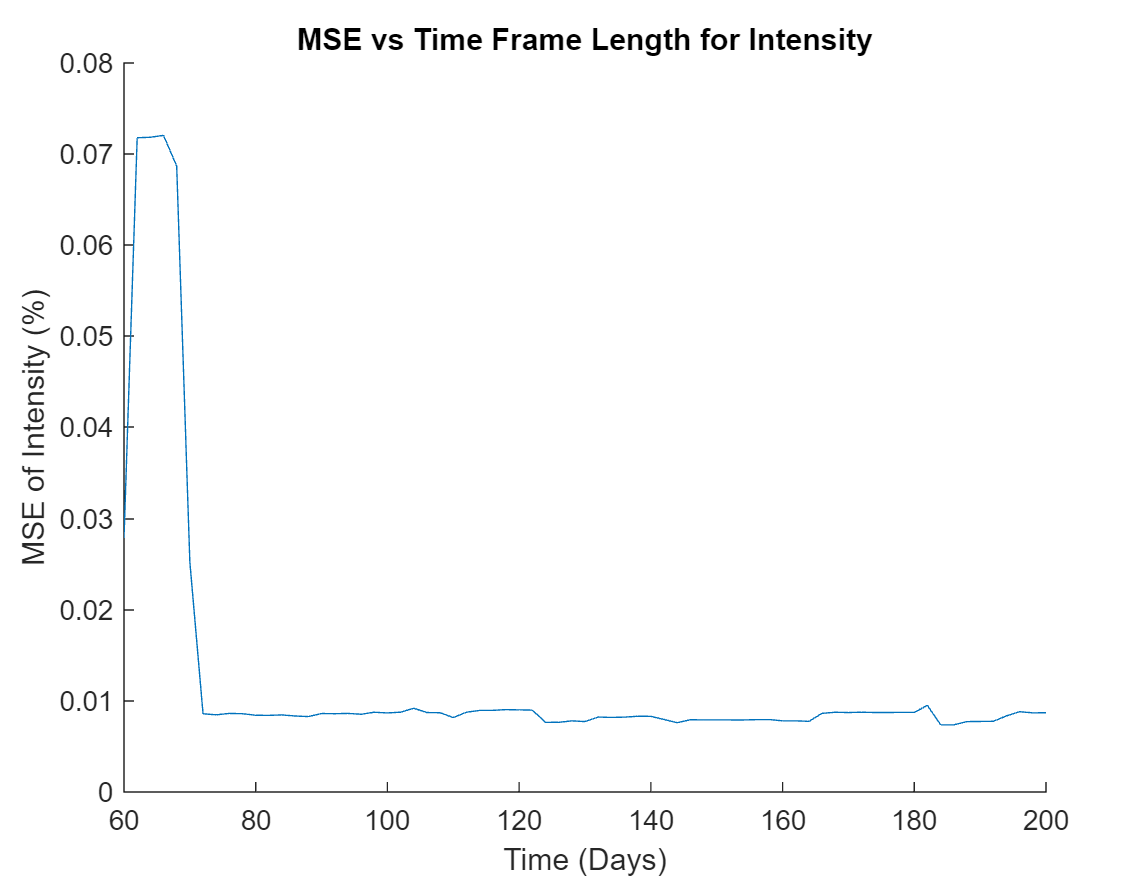
\includegraphics[width=140mm]{ActualVsPredValues/MSEvsStaticTimeFrame.png}
    \caption{The MSE over for intensity given different values of $t_f$. Note how the first minimum is not the global minimum within the context of this graph.}
    \label{fig:MSEStaticTimeFrame}
\end{figure}

Other than the obvious time complexity issues, a static time frame has other drawbacks that are more pertinent to the models behavior. In essence, the algorithm in listing \ref{lst:StaticTimeFrameFormula} will find the time frame that minimizes error across all time values greater than the target time. This results in the model finding a value for $t_f$ that minimizes error for all times greater than $t_t$, measuring accuracy in terms of the models \textit{global accuracy}. However, measuring accuracy this way violates the models efforts to adapt to the lifters current abilities. A static time frame may fail to capture changes, especially if changes are abrupt, or it may adapt to slowly, especially if the time frame is to long. If the lifters abilities change over time, then so to should the length of the time frame, thereby allowing changes in a lifters abilities to be more easily expressed.

\section{Choosing A Time Frame: Dynamic Time Frame Analysis}
\label{sec:TimeFrameDynamicTimeFrameAnalysis}

If the length of the time frame is allowed to vary over time it will give the model more freedom to adapt to the lifters current abilities. Much of the setup will remain the same from section \ref{sec:TimeFrameStaticTimeFrameAnalysis}, with equation \ref{eq:ValidTimeFrameSet} remaining valid in this section.  Figure \ref{fig:DynamicTimeFrameDiagram} demonstrates the process of selecting a dynamic time frame.

The algorithm to find a dynamic time frame is shown in listing \ref{lst:DynamicTimeFrameFormula}. The general idea of the algorithm is to select a time frame that minimizes the error of the closest data before the target time, and then that time frame can be used to predict the intensity at the target time. The main difference between the static and dynamic algorithms is the dynamic algorithm only measures accuracy in terms of the target time, and not in terms of every time before the target time. This results in the dynamic algorithm using the square error (SE) instead of the MSE to calculate accuracy for each individual target time. Once the SE is found for each target time the MSE can then be found across all target times. In essence, the dynamic time frame approach is only concerned with \textit{local accuracy}, whereas the static time frame approach is concerned with global accuracy.

\begin{figure}[h]
    \centering
    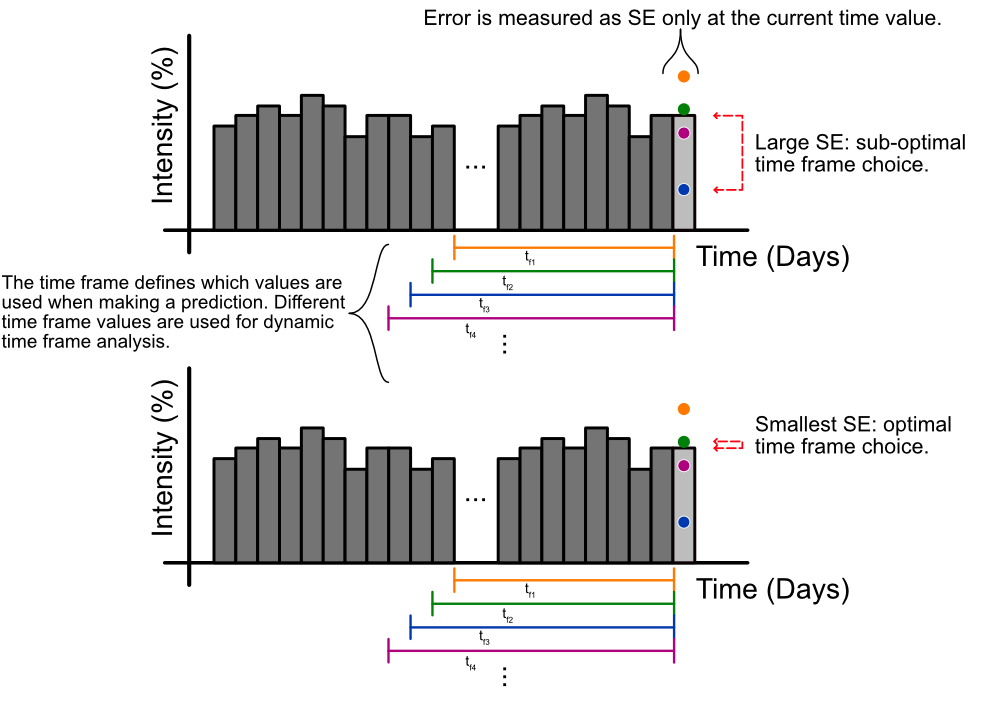
\includegraphics[width=150mm]{Diagrams/DynamicTimeFrameDiagram.png}
    \caption{A diagram showing how a dynamic time frame is calculated from the data set.}
    \label{fig:DynamicTimeFrameDiagram}
\end{figure}

A side effect of only measuring accuracy locally is an improved time complexity. The algorithm shown in listing \ref{lst:DynamicTimeFrameFormula} has a time complexity of $O(n^2)$, which is better than the $O(n^3)$ time complexity of the comparable static algorithm. This is also true for the algorithm to find historical data, with the dynamic algorithm shown in listing \ref{lst:HistoricalDynamicTimeFrameFormula} having a time complexity of $O(n^3)$. Obviously, these time complexities are still not great but it is a step in the right direction.

A dynamic programming approach similar to the one used in the static algorithm can also be used in listing \ref{lst:DynamicTimeFrameFormula} to reduce it's time complexity to $O(n)$. A linear time complexity is manageable, making the dynamic algorithm a viable way to select a time frame. This also reduces the time complexity of \ref{lst:HistoricalDynamicTimeFrameFormula} to be $O(n^2)$, which is not great, but can still be used to generate recent historical data.

Of course, only measuring accuracy locally does have some negative effects. Only measuring accuracy locally means that less information about the models performance is available when compared to the static algorithm. This is shown in the return values in listings \ref{lst:StaticTimeFrameFormula}-\ref{lst:HistoricalDynamicTimeFrameFormula}, with less information being returned from the dynamic algorithms. This is not a major concern however, as the accuracy of the model can still be assessed with the output of the dynamic algorithm.

\begin{minipage}{\linewidth}
\begin{lstlisting}[caption={The algorithm that describes how to exhaustively find a dynamic time frame's length such that it minimizes the models error.},label={lst:DynamicTimeFrameFormula},mathescape=true]
# $s$, $r$, $E$, $F$, and $t$ are all lists of there respective variables
fun dynamicTimeFrame$(s,r,E,F,t,t_t) \to \left( t_{f}, d_{iff} \right)$
    $t_{f,min}=0$
    $d_{iff,min}=\infty$
    $M_{min}=\{\}$
    for each $t_{f,i}\in \{ t_f \; | \; t_{t+1}+t_f\le \max_{t_1\dots t_n}(t) \} $
        # The $t+1$ subscript ensures the current data point, the value being
        # predicted, is not part of the model state
        $M=$modelState$(t_{t,i+1},t_{f,i})$
        $I_{pred}=$intesityPrediction$(M,s_{t+1},r_{t+1},E_{t+1},F_{t+1})$
        $d_{iff}=(I_{pred}-I_{t+1})^2$
        if $d_{iff}<d_{iff,min}$
            $\left( d_{iff,min}, t_{f,min}, M_{min} \right)=\left(  d_{iff}, t_{f,i}, M \right)$
    return $(t_{f,min},(\texttt{intensityPrediction}(M_{min},s_t,r_t,E_t,F_t)-I_t)^2)$
\end{lstlisting}
\end{minipage}

\begin{minipage}{\linewidth}
\begin{lstlisting}[caption={The algorithm that describes how to find historical dynamic time frames.},label={lst:HistoricalDynamicTimeFrameFormula},mathescape=true]
# $s$, $r$, $E$, $F$, and $t$ are all lists of there respective variables
fun historicalDynamicTimeFrames$(s,r,E,F,t) \to \left( [t_{f,1},\dots,t_{f,n}], \varepsilon \right)$
    $d_{iff}=[\infty, \infty, \dots]$ where $|d_{iff}|=|t|$
    $t_{f,min}=[0, 0, \dots]$ where $|t_{f,min}|=|t|$
    for each $t_{t,i}\in \{ t \}$
        $(t_{f,min}[i],d_{iff}[i])=$dynamicTimeFrame$(s,r,E,F,t,t_{t,i})$
    return $($
        $t_{f,min}$,
        $\texttt{sum}(
            \texttt{filter}(d_{iff},\texttt{val}!=\infty)
        )/
        \texttt{count}(
            \texttt{filter}(d_{iff},\texttt{val}!=\infty
        )$
    $)$
\end{lstlisting}
\end{minipage}

Figure \ref{fig:PredictionsVsActualDynamicTimeFrame} is the result of running the dynamic time frame algorithm on deadlift data. Note how the MSE has decreased to $0.42\%$ compared to $0.78\%$ from the static algorithm. Put another way: using a dynamic time frame the model is, on average, within $0.42\%$ of the actual intensity. Other than the increased accuracy, another thing of note is the increased range over which predictions were able to be made compared to the static time frame shown in table \ref{tab:PredictionsVsActualConstantTimeFrame}. This is because the models time frame was able to shrink when it butted up against the end of the data set in the dynamic approach, whereas in the static approach if the time frame went past the end of the data set no predictions could be made.
%and figure \ref{fig:TimeFrameAcrossTime} shows the time frame length across time

\begin{figure}[h]
    \centering
    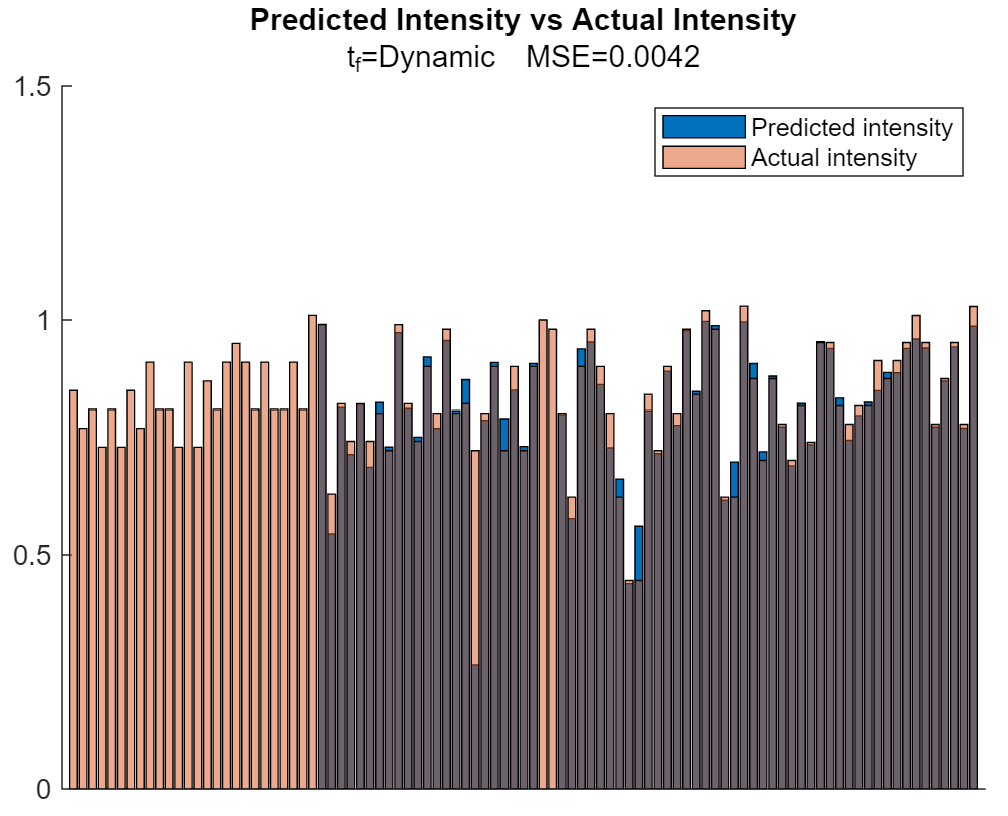
\includegraphics[width=120mm]{ActualVsPredValues/DynamicTimeFrameActualVsPredIntensity.png}
    \caption{Predicted values compared to actual values for intensity using deadlift data. Note how using the dynamic time frame extended the range of values that have predictions while still having higher accuracy.}
    \label{fig:PredictionsVsActualDynamicTimeFrame}
\end{figure}
%\begin{figure}[h]
%    \centering
%    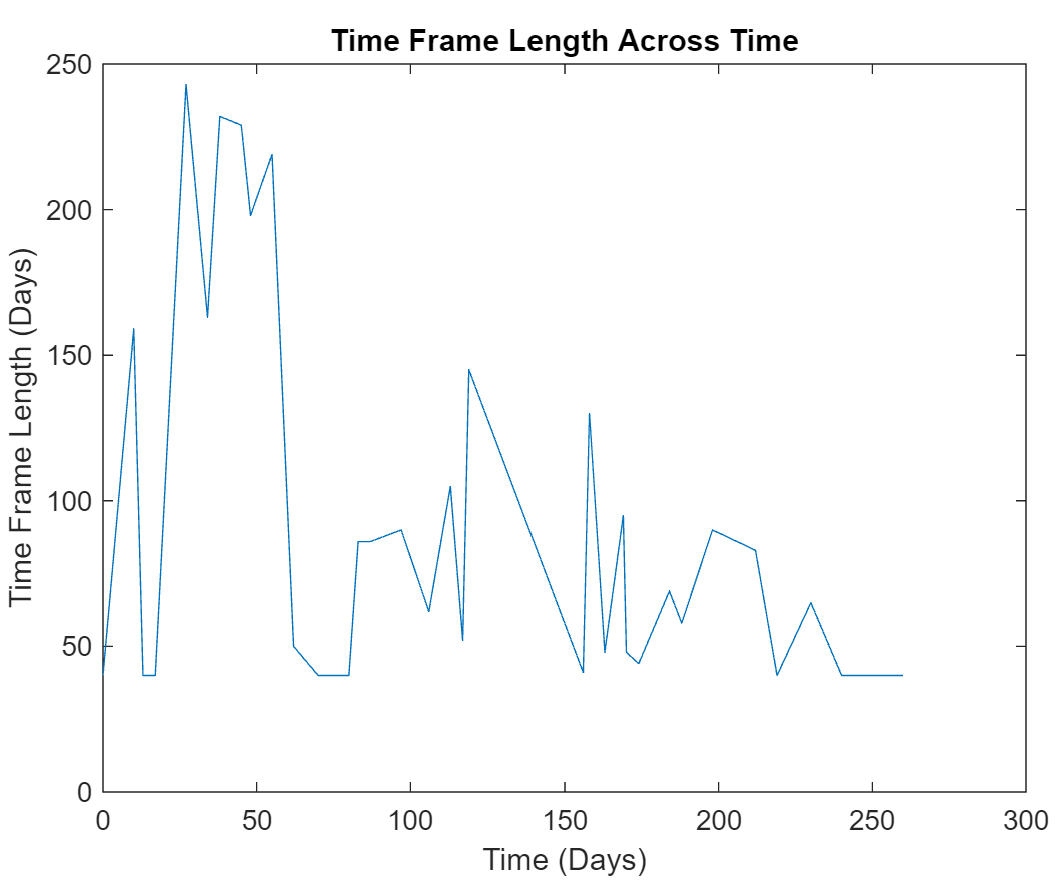
\includegraphics[width=120mm]{DeadliftConstants/TimeFrameLengthAcrossTime.png}
%    \caption{Time frame length over time. Note the general trend of increasing time frames, which is partly a function of the model having more data to work with as $t_t\to 0$.}
%    \label{fig:TimeFrameAcrossTime}
%\end{figure}

%TODO - add plot showing updated 1RM predictions

\section{Choosing A Time Frame: The General Case Through Sliding Window Analysis}
\label{sec:TimeFrameSlidingWindowAnalysis}

It turns out that the two 

\section{Analysis: Injuries, Setbacks, and Changes}
\label{sec:TimeFrameInjuriesAndChanges}

Section \ref{sec:TimeFrameDynamicTimeFrameAnalysis} was concerned with allowing the model to better adapt to a lifters current abilities. Using a 'local' measure of accuracy seemed to allow this, but proof that it does is needed.

An obvious place to check if the model is adapting to the lifters current abilities is the dates surrounding the lifters injury on $3/3/2022$. After an injury the model should respond by reducing the time frame so that only recent data is included, reflecting any drop in performance. A second place to check where the model adapts to a lifters current abilities is the dates surrounding any 1RM attempt. If the lifter peaked properly for the attempt then the models time frame should decrease leading up to the attempt and then re-increase again afterwards.

Looking at the time frame from $3/27/2022$-$5/30/2022$ the aforementioned patterns are present. The relevant data points and there respective time frames shown in table \ref{tab:TimeFrameNearCompetitionDeadlift}. From $3/27/2022$-$4/9/2022$ the time frame is trending downwards, indicating the model is adapting to the lifters post-injury capabilities. From $4/9/2022$-$4/28/2022$ the time frame re-increases, indicating the lifters abilities are returning. From $4/28/2022$-$5/5/2022$ the time frame decreases as the lifter approaches the competition on $5/5/2022$. Then, after the competition the time frame increases again. The behaviors of the time frame from table \ref{tab:TimeFrameNearCompetitionDeadlift} show the model is adapting to the lifters current abilities.

%An example of this is from the deadlift data between the dates of $4/2/2022$ and $5/30/2022$. The relevant data points and there respective time frames shown in table \ref{tab:TimeFrameNearCompetitionDeadlift}. Notice how as the competition approaches the models time frame begins to decrease, and afterwards the time frame re-increases. This is because the model was picking up on the lifters peak leading into the competition, where performance is temporarily boosted due to decreased fatigue levels.

\begin{table}[h]
    \centering
    \begin{tabular}{c|c}
        Date & $t_f$ \\
        \hline
        $3/27/2022$ & $145$ \\
        $3/29/2022$ & $52$ \\
        $4/2/2022$ & $105$ \\
        $4/9/2022$ & $62$ \\
        $4/18/2022$ & $90$ \\
        $4/28/2022$ & $86$ \\
        $5/2/2022$ & $86$ \\
        $5/5/2022$ & $40$ \\
        $5/15/2022$ & $40$ \\
        $5/23/2022$ & $50$ \\
        $5/30/2022$ & $219$
    \end{tabular}
    \caption{Time frame length over time when a lifter was peaking for a competition on $5/5/2022$. Notice how the time frame decreases as the competition approaches and then re-increases. This is proof the model can capture recent changes in training.}
    \label{tab:TimeFrameNearCompetitionDeadlift}
\end{table}

If an injury is severe enough, a lifter may loose all training progress and may never be capable of the same performance ever again. The data set (thankfully) does not have any data relating to a case like this, which makes it difficult to assess how quickly the model would respond to such a scenario. Even if the model does not respond quickly however, it does not make sense to include any data from the time before the injury occurred. To ensure this does not happen, the time frame can be limited to only include data from after the injury, creating a clean slate for the model to re-learn the lifters new abilities.

\section{Application: Predicting the Future?}
\label{sec:TimeFramePredictingTheFuture}

Up until now, the model was only making predictions about the current day. The next natural question is can the model make predictions further in the future? The answer is yes, but only based on the models current state. This is a pretty big 'but', as the models state will have changed by the time any future date is reached, thereby changing any predictions it would have made. To further complicate the issue, the more data is added to the data set between the current time and the predicted time the greater the potential is for the model state to vary drastically. This generally means the further out a prediction is in the future the less accurate it will be, and it is this reason that the predictions have been limited to only capture the next training session, and not reach beyond that. However, if changes to the models state can be predicted over time, then more valid predictions can be made about the future.

%TODO - make plot showing how this happens

%The next chapter will deal with finding patterns in the changing of state - a meta analysis